  \begin{minipage}[b]{0.5\linewidth}
    \begin{tikzpicture}
      \tikzstyle{every state}=[fill=purple, text=white, draw=none]
      \node[state, scale=0.5] (A) at (0, 0) {\large{$0$}};
      \node[state, scale=0.5] (B) at (1, 1) {\large{$1$}};
      \node[state, scale=0.5] (C) at (1, -1) {\large{$2$}};
      \node[] at (0,1.25)   {\footnotesize{$\left(-2, 0, 0\right)$}};
      \node[] at (-1,-0.5)  {\footnotesize{$\left(-\frac{\sqrt{5}}{2}, 0, -\frac{2\pi}{3}\right)$}};
      \node[] at (1, 0.5)   {\footnotesize{$\left(2, 0, 0\right)$}};
      \node[] at (1.2, -0.25)  {\footnotesize{$\left(-\frac{1}{2}, 1, \frac{2\pi}{3}\right)$}};
      \draw[arc] (A) to[out=45, in=-135] (B);
      \draw[arc] (A) to[out=-45,in=135] (C);
      \draw[arc] (C) to[out=180, in=-90] (A);
      \draw[arc] (B) to[out=180, in=90] (A);
    \end{tikzpicture}
  \end{minipage}
\begin{minipage}[b]{0.4\linewidth}
    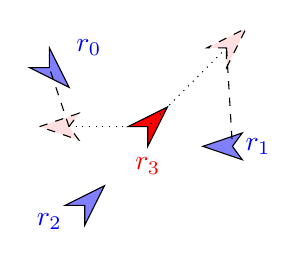
\begin{tikzpicture}
      \draw[fill=blue!50] (3.2,3) -- (2.95,3) -- (3.45,3.25) -- (3.2,2.75)   -- cycle;
      \node[color=blue] at (2.75, 2.8) {$r_2$};
      % draw grids
      % \draw[color=gray, help lines, line width=.05pt] (-1,1)  grid[xstep=.5cm, ystep=.5cm] (6,6);
      \draw[fill=blue!50] (3,4.5) -- (2.75,5) -- (2.75,4.75) -- (2.5,4.75)   -- cycle;
      \node[color=blue] at (3.25, 5) {$r_0$};
      \draw[fill=blue!50] (5.2,3.92) -- (4.7,3.75) -- (5.2,3.58) -- (5.075,3.75)  -- cycle;
      \node[color=blue] at (5.4,3.75) {$r_1$};
      \draw[fill=red] (4,4) -- (3.75,4) -- (4.25,4.25) -- (4,3.75) -- cycle;
      \node[color=red] at (4, 3.5) {$r_3$};
      \draw[dashed, fill=pink!50] (3,4)  -- (3.125,4.17) -- (2.625,4) -- (3.125,3.83) -- cycle;
      \draw[dotted] (3,4) -- (4,4);
      \draw[dashed, fill=pink!50] (5,5) -- (4.75,5) -- (5.25,5.25) -- (5,4.75) -- cycle;
      \draw[dotted] (5,5) -- (4,4);
      \draw[dashed] (5,5) -- (5.075, 3.75);
      \draw[dashed] (3,4) -- (2.75,4.75);
    \end{tikzpicture}
  \end{minipage}

\caption{Assume the range $\range=2$. [left] A lattice graph consists of three nodes. [right] The robot $r_3$ has $3$ neighbors $r_0, r_1, r_2$. Robot $r_3$ is the root of the authority tree, $r_0, r_1, r_2$ are the descendants of $r_3$. According to the lattice graph on the left, the role of $r_3$ is $0$, it matches $r_0$ and $r_1$ to two destinations (dashed). Robot $r_2$ is assigned the null value $g(r_2)=\emptyset$ by $r_3$.}
